\documentclass{sig-alternate}

\usepackage{todonotes}
\usepackage{hyperref}
\usepackage{amssymb}
\usepackage{amsmath}
\newcommand{\mytodo}[1]{\textbf{[[#1]]}}

\begin{document}
%
% --- Author Metadata here ---
\conferenceinfo{Foundations of Digital Games}{???}
%\CopyrightYear{2007} % Allows default copyright year (20XX) to be over-ridden - IF NEED BE.
%\crdata{0-12345-67-8/90/01}  % Allows default copyright data (0-89791-88-6/97/05) to be over-ridden - IF NEED BE.
% --- End of Author Metadata ---

\title{Automatic Playtesting for Game Parameter Tuning via Active Learning}


\numberofauthors{1} 

\author{
\alignauthor
anonymous
%Alexander Zook and Mark O. Riedl\\
%       \affaddr{School of Interactive Computing, College of Computing}\\
%       \affaddr{Georgia Institute of Technology}\\
%       \affaddr{Atlanta, Georgia, USA}\\
%       \email{\{a.zook, riedl\}@gatech.edu}
}


\maketitle
\begin{abstract}
Game designers often use human playtesting to gather feedback about game design elements when iteratively improving a game.
Playtesting, however, is expensive: human testers must be recruited, playtest results must be aggregated and interpreted, and changes to game designs must be extrapolated from these results.
We argue that active learning techniques can be used to formalize and automate a subset of playtesting goals.
Specifically, we focus on the low-level parameter tuning required to balance a game once the mechanics have been chosen.
Through a case study on a shoot-`em-up game we demonstrate the efficacy of active learning to reduce the amount of playtesting needed to choose the optimal set of game parameters for a given (formal) design objective.
This work opens the potential for additional methods to reduce the human burden of performing playtesting for a variety of relevant design concerns.
\end{abstract}

% A category with the (minimum) three required fields
\category{\todo[inline]{pick}H.4}{Information Systems Applications}{Miscellaneous}
%A category including the fourth, optional field follows...
\category{D.2.8}{Software Engineering}{Metrics}[complexity measures, performance measures]

\terms{\todo[inline]{pick}}

\keywords{\todo[inline]{pick}}

\section{Introduction}

\todo[inline]{update top part w/FDG info}


% motivation
Iterative game design practices emphasize the centrality of playtesting to improve and refine a game's design.
Human playtesters provide valuable feedback on audience reactions to a game.
Playtesting is often claimed to be ``the single most important activity a designer engages in'' \cite{fullerton2008:playcentric}.
Test data informs designers of how real players may react to the game in ways that self-testing, simulations, and design analysis may not.
Playtesting, however, is expensive---developers must recruit players, devise design experiments, collect game play and subjective feedback data, and make design changes to meet design goals.

%  other quotes:
%``You might be thinking: But testing is an expensive process, isn't it?'' p.248

% problem
We ask the question: can we reduce the cost of the playtesting process by automating some of the more mundane aspects of playtesting?
To address this problem we focus on a subset of playtesting questions focused on ``parameter tuning.''
Parameter tuning involves making low-level changes to game mechanic settings such as character movement parameters, power-up item effects, or control sensitivity.
Games based on careful timing and reflexes depend on well-tuned parameters, including racing, platforming, shoot-`em-up, and fighting game genres.
Addressing the problem of parameter tuning requires a means to automatically select a set of potentially good parameter settings, test those settings with humans, evaluate the human results, and repeat the process until a pre-defined design goal is achieved.


% contributions
Our central insight is to model playtesting as a form of active learning.
Active learning \cite{settles2012:al-book} involves selecting among a set of possible inputs to get the best output while minimizing the number of inputs tested.
We define the ``best output'' in terms of a parameter tuning design goal and treat a setting for a game design as an ``input.''
This paper makes three contributions toward machine-driven playtesting:
\begin{enumerate}
\item Machine-driven playtesting---a formulation of efficient playtesting as an active learning problem % TODO: "active playtesting"? "machine-driven playtesting"? needs a better name
\item A definition of a set of playtesting goals in terms of active learning metrics
\item A case study of a shoot-`em-up game demonstrating the efficacy of active learning to reduce the number of playtests needed to optimize (1) difficulty-related and (2) control-related game parameters
\end{enumerate}

% differences from prior work
Unlike prior work in dynamic difficulty and adaptive games we focus on the case of deciding on a fixed design for future use.
Our approach can be applied to online game adjustments to more rapidly converge on the right set of game parameters.
%Further, by learning a model of how design parameters influence playtest results our approach is able to provide designers additional feedback on their ``design space'' at design time.
%A design space can be visualized to understand the tradeoffs among different parameter settings.
Unlike prior work on game design support tools using simulations or model-checking we focus on the problem of efficiently working with a set of human testers.
Our approach complements these tools for early-stage testing with late-stage refinement.

% roadmap
In the remainder of the paper we first compare our approach to related efforts at game design support.
We next define a set of parameter tuning design goals and relate them to active learning approaches.
Following this we describe a case study of automated playtesting using a shoot-`em-up game.
After describing the game used we present results showing the efficacy of active learning to model a known simulated player model and human data collected from an online study.
We conclude with a discussion of the limitations, applications, and potential extensions to this playtesting approach.



%%%%%%%%%%%%%%%%%%%%%%%%%%%%%%%%%%%

\section{Related Work}

% overview
Two research areas are closely related to automated playtesting: offline game design tools and online game adaptation.
Offline game design tools enable designers to explore possible game designs by defining a high-level space of games through a design language.
Examples include support for generating or evaluating design in terms of hard constraints (what must be true) or soft optimization (what to achieve to the best degree possible).
Offline game design tools enable designers to explore possible game designs by defining a high-level space of games through a design language.
Examples include support for generating or evaluating design in terms of hard constraints (what must be true) or soft optimization (what to achieve to the best degree possible).



\subsection{Offline Game Design Tools}
% offline design: model-checking vs simulation
Offline game design tools have evaluated game designs using simulated players and formal model-checking.
Simulation-based tools use sampling techniques to test aspects of a game design for ``playability,'' typically defined as the ability for a player to reach a given goal state with the current design parameters.
Model-checking tools define game mechanics in a logical language to provide hard guarantees on the same kinds of playability tests.

% simulation
Bauer et al. \cite{bauer2013:rrt-generation} and Cook et al. \cite{cook2012:coopcoevo} use sampling methods to evaluate platformer game level playability.
Shaker et al. \cite{shaker2013:ropossum-test} combine a rule-based reasoning approach with simulation to generate content for a physics-based game.
Simulation approaches are valuable when design involves an intractably large space of possible parameters to test and can serve as input to optimization techniques.
Active learning can enhance simulation approaches by guiding the sampling process toward spaces of parameters likely to be of greater value.

% model-checking
Model-checking approaches provide guarantees on generated designs having formally defined properties---typically at the cost of being limited to more coarse design parameter decisions.
Smith et al. \cite{smith2013:quantify-play}, Butler et al. \cite{butler2013:progression-tool}, and Horswill and Foged \cite{horswill2012:levelgen} employ logic programming and constraint solving to generating levels or sets of levels meeting given design constraints.
Jaffe et al. \cite{jaffe2012:balance} employ game-theoretic analysis to understand the trade-offs of game design parameters for balance in a competitive game.

% differences of playtest vs model-check -> value to designers
Our approach to automated playtesting is intended to complement these approaches to high-level early design exploration with low-level optimization of game parameters and tuning.
Further, we focus on a generic technique that applies to cases with human testers in the loop, crucial to tuning game controls or subjective features of games.
%
Offline design tools currently enable designers to formally define and enforce properties of a game design across all possible player behaviors in a specific game or space of designs.
To date these tools have emphasized techniques for ensuring game designs have desired formal properties that meet designer intent.
%
% note: not about model-checking vs playtesting but expanding offline tools available
Machine-driven playtesting enables players to provide feedback to designers on \textit{expected} player behaviors in a game.
Developing machine-driven playtesting techniques affords designers insight into how human audiences interact with designer intent, complementing an understanding of whether and how a game matches formal criteria.




\subsection{Online Game Adaptation}
%% online adaptation: hand-crafted rules vs ML/EC
% hand-crafted rules
Online game adaptation researchers have used both hand-crafted rules and data-driven techniques.
Hunicke and Chapman \cite{hunicke2004:dda} tracked the average and variance of player damage and inventory levels and employ a hand-crafted policy to adjust levels of enemies or powerups. 
Systems by Magerko et al. \cite{magerko2006:isat}, El-Nasr \cite{seifel-nasr2007:mirage}, and Thue et al. \cite{thue2007:storytell-pm} model players as vectors of skills, personality traits, or pre-defined ``player types'' and select content to fit players using hand-crafted rules. % note: erring on side of more for now
Hand-crafted rules enable designers to describe fine-tuned details of how to adjust a game toward design goals.
However, designers must fully describe how to tune the game and rules are often sensitive to minor changes in game settings.

% ML / EC
To bypass the brittleness of rules others have employed data-driven techniques that optimize game parameters toward design goals.
Hastings et al. \cite{hastings2009:gar}, Shaker et al. \cite{shaker2013:crowdsource-platform-aesthetics}, Liapis et al. \cite{liapis2013:rank-based-interactive-evol} and Yu and Riedl \cite{yu2013:storyeti} model player preferences using neuro-evolutionary or machine learning techniques and optimize the output of these models to select potential game parameters.
Harrison and Roberts \cite{harrison2013:scrabble-retention} optimize player retention and Zook and Riedl \cite{zook2012:tf} optimize game difficulty using similar techniques.

%Both rule-based and data-driven online adaptation approaches target real-time adjustments of a game to known design goals.
Automated playtesting extends these approaches by providing principled methods for guiding the process of designing hand-crafted rules or optimizing game parameters.
When hand-crafting rules, automated playtesting informs the choice of which rule parameters to use.
When optimizing models learned from data, automated playtesting informs the choice of which next set of parameters to test during the optimization process.
We argue that research to date has ignored the problem of reducing ``sample complexity''---the number of data points (human tests) needed to train a model.
Active learning makes explicit the trade-off in playtesting between ``exploring'' potentially valuable game design settings and ``exploiting'' known good solutions with small changes.
%Active learning complements the above approaches by providing a principled method for reducing the number of playtests needed without changing the fundamental models involved.
Thus, active learning complement online game adaptation through reducing the number of mediocre or bad sets of game parameters players experience before arriving at good parameter settings without changing the underlying models used.



%%%%%%%%%%%%%%%%%%%%%%%%%%%%%%%%%%

\section{Active Learning}

Our goal is to reduce the playtesting burden by efficiently choosing game designs to test on players.
Active learning (AL) provides a generic set of techniques to guide the playtesting process of choosing a set of design parameters to test toward achieving a design goal.
Playtesting typically involves trade-offs between testing designs that are poorly understood (exploration) and refining designs that are known to be good but need minor changes (exploitation).
Active learning captures this intuition through explicit models of the exploration-exploitation trade-off.
In the following sections we will define active learning in the playtesting context and provide the intuition behind several common active learning methods.
Our aim is to characterize playtesting in terms of active learning; full mathematical treatments are available through the references.


\subsection{Playtesting as Active Learning}
Machine-driven playtesting---AL for game design---uses a model of how a design works to choose how to change that design to achieve a design goal.
Formally, the design goal is known as the \textit{objective function} and captures the relationship between input (game design parameters) and desired output (game design goals).
An \textit{acquisition function} takes information on expected outputs from the objective function and uses it to decide on the next set of inputs to test.

Objective functions come in two forms: regression and classification models.
\textit{Regression} models capture continuous outputs---e.g. how the rate of enemy firing in a shoot-`em-up influences the number of times a player is hit or how the height of jumps in a platformer influences how long it takes players to complete a level.
\textit{Classification} models capture discrete outputs---e.g. whether a player preferred the current control sensitivity compared to the previous set of controls in a racing game or which choice a player made in a choose-your-own adventure.
Note that many design goals can be formulated as goals for playtesting: the primary challenge lies in defining a useful metric for measuring these goals through player feedback or in-game behavior.


Acquisition functions differ for regression and classification functions.
In the next sections we provide intuitive definitions of several acquisition functions---references to the relevant mathematical literature are provided.
Our survey of regression methods covers key methods that balance between exploration of possible designs and exploitation to refine high quality designs.
For classification methods we cover the two most common frameworks for AL with discrete data that are intended to mitigate the impact of highly variable data.



\subsection{Regression Models}
%% regression
We consider four acquisition functions for regression models: (1) variance, (2) probability of improvement, (3) expected improvement, and (4) upper-confidence bounds.
% variance
The \textit{variance} acquisition function picks designs based purely on the uncertainty of the design goal value \cite{brochu2010:thesis}.
Intuitively, variance encodes a playtesting strategy of attempting any design that is poorly understood until the entire design space is well-understood.
Variance approaches are pure exploration and are useful when design information on many possibilities is needed.

% probability of improvement
\textit{Probability of improvement} (PI) improves on uncertainty by selecting the design that is most likely to gain some improvement of the best design observed so far \cite{brochu2010:thesis}. 
Intuitively, probability of improvement is a playtesting strategy of attempting the design that seems most likely to improve over what has been tried so far.
Probability of improvement approaches are pure exploitation and are effective when performing minor tweaks to already-effective designs.

% expected improvement
\textit{Expected improvement} (EI) enhances PI by weighting the probability of each design improvement by the amount of improvement \cite{brochu2010:thesis}.
Unlike probability of improvement or variance, EI balances between exploration and exploitation.
Intuitively, EI seeks designs that are likely to have large improvements over the existing design.
%Mathematically EI is typically very computationally expensive, though for certain objective functions it has analytic solutions that are readily used.
%Below we use one such objective function, the Gaussian Process \cite{rasmussen2006}.
By balancing exploration and exploitation EI is a more general-purpose technique useful for playtesting during many stages of the development cycle.

% upper confidence bounds
\textit{Upper Confidence Bound} (UCB) methods select designs based on the upper bound on design quality according to a model of design quality and variability in that quality \cite{srinivas2010:gp-ucb}.
Designs that are expected to be high quality but are also poorly understood (and thus highly variable) are given priority.
By testing these designs UCB narrows down the space of designs to those known to be good or unknown but likely to be bad.
In the UCB approach cited above the importance of variability is gradually scaled down as more playtests are run.
Intuitively, this capture the notion of initially exploring a variety of possible designs and gradually converging to exploit the most promising designs.

% some kind of wrap-up?


\subsection{Classification Models}
%% classification
We consider three acquisition functions for classification models: (1) entropy, (2) query-by-bagging voting, and (3) query-by-bagging probability.
% entropy
% note: technically a subset of uncertainty sampling
% (1) least confident
% (2) margin-based
% (3) entropy
\textit{Entropy} acquisition functions choose designs that are most uncertain according to entropy \cite{settles2012:al-book}.
Entropy measures the amount of information needed to encode a distribution.
Intuitively, this captures how uncertain a model is about the possible (discrete) outcomes.
Entropy sampling acts similarly to variance-based sampling for regression.


% QBB
% note: technically a subset of query-by-committee
% (1) QBC
% (2) QBB
\textit{Query-By-Bagging} (QBB) approaches emphasize disagreement among potential models \cite{settles2012:al-book}.
First, multiple copies of the same objective function are trained using random selections of the playtest data gathered so far.
This captures the notion of guessing how the model might be if slightly different sets of playtests had occurred.
Second, these models predict the outcome of new playtests.
The final choice of design to test is the one these models most disagree on.
Intuitively, this captures the idea of picking designs that are most likely to be poorly understood.

% QBB vote
% QBB probability
Two varieties of QBB are relevant: QBB vote and QBB probability.
In \textit{QBB vote} each objective function model votes on outcomes, giving a single choice.
When only two options are possible (e.g. controls were better or worse) the design with the greatest disagreement between two binary outcomes is chosen.
%% TODO: verify me with actual tests!
When multiple options are possible (e.g. a multi-way branch in a choose-your-own-adventure), the design with the greatest difference between the top two options is chosen.
%
In \textit{QBB probability} each objective function model estimates how probable each outcome is, giving a weight to all choices.
The weights of all models are averaged and the point with lowest probability is chosen. \todo[inline]{find citation}

% TODO: KL-divergence or vote entropy?

% TODO: decision boundary distance for KSVM?

% TODO: more of uncertainty sampling?

% TODO: error reduction methods?


%%%%%%%%%%%%%%%%%%%%%%%%%%%%%%%%%%%%%

\section{Game Domain}

\begin{figure}[t]
\centering
%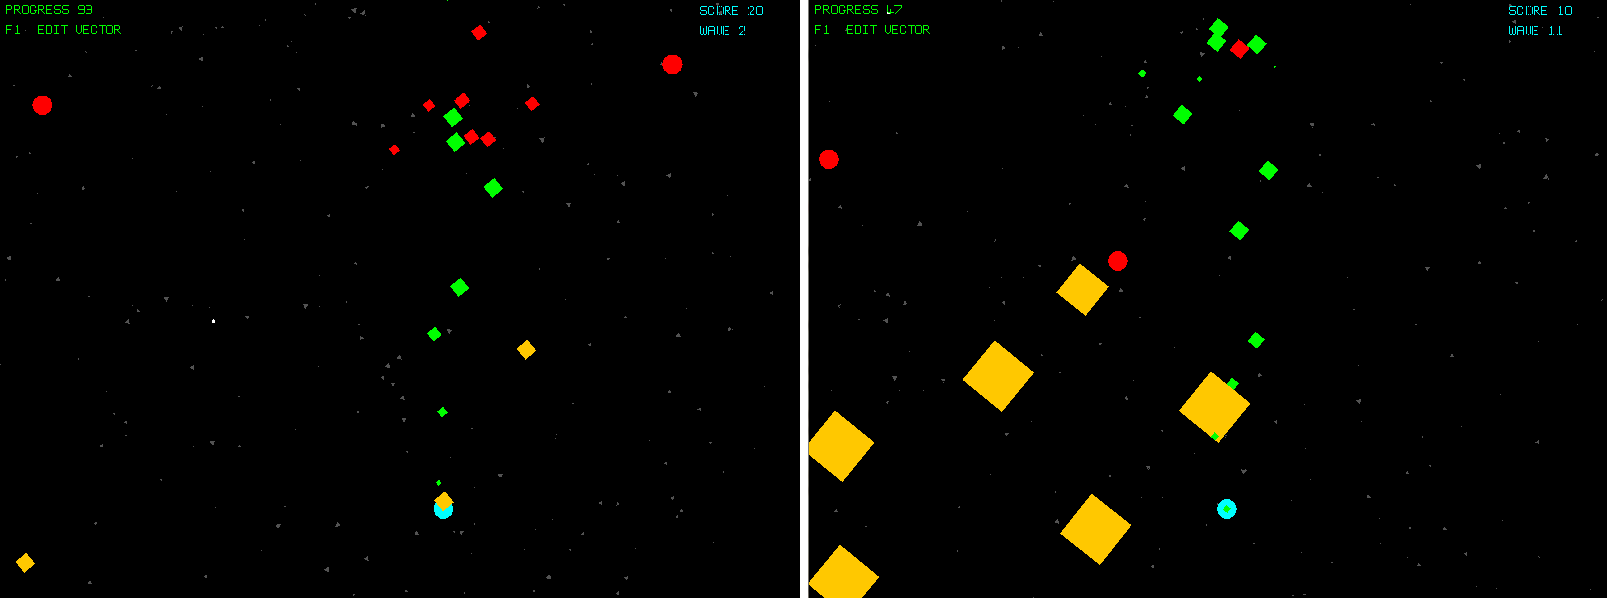
\includegraphics[width=1\linewidth]{./bullethell_sidebyside}
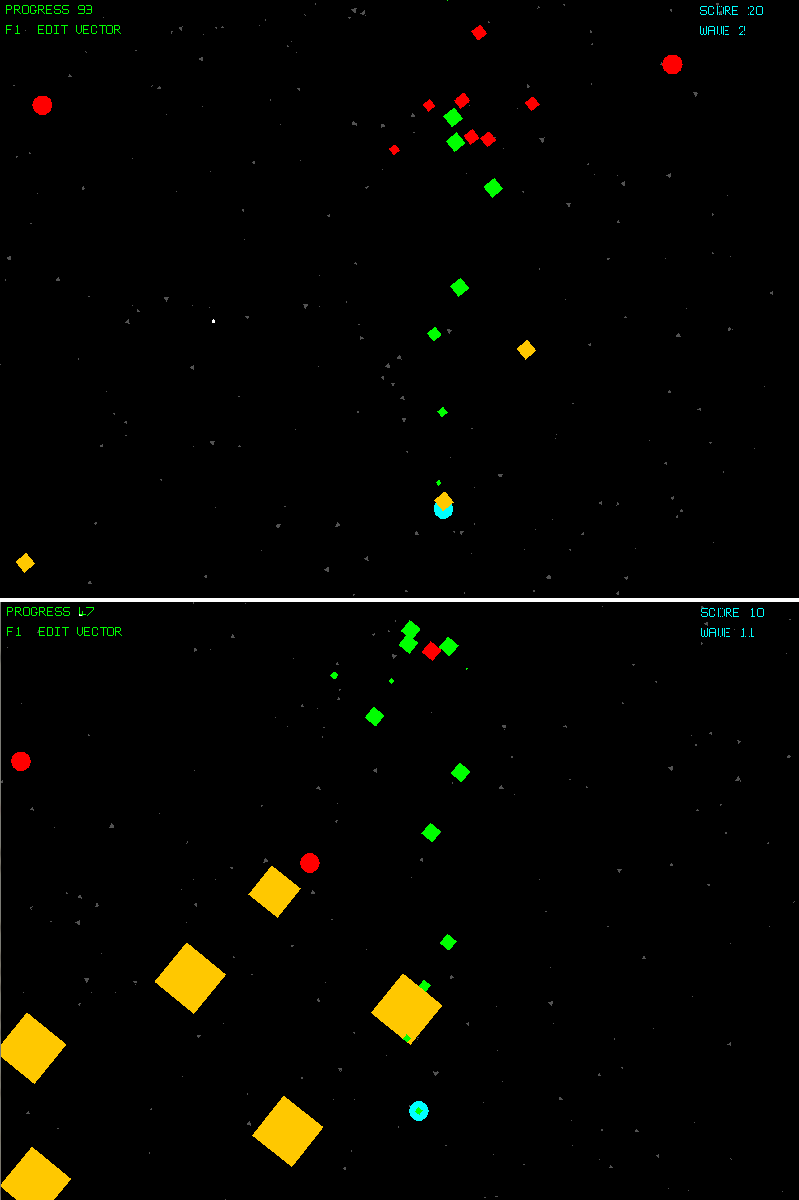
\includegraphics[width=1\linewidth]{./bullethell_topbybottom}
\caption{Study game interface illustrating player, enemies, and shots fired by both at two points along adaptation process.}
%Preference learning experiments varied parameters related to player movement; enemy tuning involved the speed, size, and rate of fire of enemy bullets.
\label{fig:shmup}
\end{figure}

In order to conduct a case study of machine-driven playtesting we developed a simple shoot-`em-up game (Figure \ref{fig:shmup}).
Shoot-`em-up games emphasize reflexes and pattern recognition abilities as a player maneuvers a ship to dodge enemy shots and return fire.
%
In general, arcade games serve as an ideal starting domain for low-level parameter tuning:
\begin{itemize}
\item There are a number of parameters that can potentially interfere with each other: size and speed of enemies and enemy bullets, rate of enemy fire, player speed, player rate of fire, etc.
\item The game can be played in a series of waves, enabling our system to naturally test game parameter settings and gather player feedback.
\item Action-oriented gameplay reduces the complexity of player long-term planning and strategizing.
\item A scoring system makes gameplay goals and progress clear, unlike domains involving puzzle-solving or aesthetic enjoyment of a game world or setting.
\end{itemize}
%
In the case of shoot-`em-up games, we tested two different kinds of game design goals: player game play behavior goals and player subjective response goals.
Player game play behavior goals cover cases where designers seek particular play patterns or outcomes---e.g. player success rates or score achieved. 
Subjective responses goals cover cases where designers desire specific player subjective feedback---e.g. getting good user ratings on the feel of the controls.


% % enemy params
The shoot-`em-up game is based on space ship combat over a series of waves.
During each wave a series of enemies appear that fire bullets at the player. 
To test active learning for regression we set a game play behavior design goal of the player being hit exactly six times during each wave of enemies and tuned enemy parameters.
We varied the: size of enemy bullets, speed of enemy bullets, and rate that enemies fire bullets. 
Increasing bullet size requires the player to move more carefully to avoid bullets. 
Faster bullets require quicker player reflexes to dodge incoming fire. 
More rapid firing rates increase the volume of incoming fire. 
Together these three parameters govern how much players must move to dodge enemy attacks, in turn challenging player reflexes. 
Getting approximate settings for these parameters is easy, but fine-tuning them for a desired level of difficulty can be challenging. 


% % control params
To test active learning for classification we set a subjective response design goal of the player evaluating a set of controls as better than the previous set and tuned player control parameters.
We varied two ship movement parameters: drag and thrust. 
Drag is the ``friction'' applied to a ship that decelerates the moving ship at a constant rate when it is moving---larger values cause the ship to stop drifting in motion sooner. 
Thrust is the ``force'' a player movement press applies to accelerate the ship---larger values cause the ship to move more rapidly when the player presses a key to move. 
%
Combinations of thrust and drag are easy to tune to rough ranges of playability.
However, the precise values needed to ensure the player has the appropriate controls are difficult to find as player movement depends on how enemies attack and individual player preferences for control sensitivity (much like mouse movement sensitivity). 
After wave of enemies a menu asked players to indicate if the most recent controls were better, worse, or as good/bad as (``neither'') the previous set of controls.
We provided a fourth option of ``no different'' for when players could not distinguish the sets of controls, as opposed to ``neither'' where players felt controls differed but had no impact on their preferences.


%Our experiments investigate how well an AI system can learn the right parameter settings to achieve a desired level of player performance (in terms of rate of being hit by enemies) or a most preferred set of controls (in terms of player subjective responses).


%%%%%%%%%%%%%%%%%%%%%%%%%%%%%%%%%%

\section{Experiments}
Our experiments sought to test whether the active learning framework could reduce the number of human playtesters needed to tune design parameters compared to a random sampling approach.
Random sampling is the standard method used to evaluate the efficacy of AL models for improving model fits for a fixed number of playtests \cite{settles2012:al-book}. This is similar to A/B testing approaches that capture large amounts of data before acting on the results.

In two experiments we used the active learning acquisition functions given above for tuning enemy parameters or tuning player controls.
Both experiments involved a preliminary test on simulated data followed by testing with human participants.
The simulation experiments allowed us to verify that our methods would work in principle; humans studies show our method can apply to real-world contexts.

In each study we employed three different objective functions---Gaussian Processes (GP), kernel support vector machines (KSVM), and optimized neural networks (``neuro-evolution'', NE).
We chose these objective functions as they cover several player modeling approaches used in this domain: GPs are a common model in active learning contexts \cite{brochu2010:thesis}, kernel methods (particularly KSVMs) are a popular machine learning technique previously used in player modeling \cite{yu2011:minboredom}, and optimized neural networks have been widely used in preference learning \cite{yannakakis2011:edpcg}.\footnote{For computational reasons we employ a simple gradient-based optimization method, rather than the more common neuro-evolutionary approaches. We did not find any performance differences between the two optimization approaches in initial tests in our domain.}
All three of these objective functions can be trained in regression or classification modes.

% enemy tuning summary
Our results show active learning can reduce the number of human playtests needed.
For enemy parameter tuning (a regression problem) we find variance, UCB, and EI are all effective in simulation, but only UCB and EI are effective on human data.
This is likely due to human players having more variability in playing behavior than our simulated models.

% control tuning results summary
For control tuning (a classification problem) we find QBB vote and entropy have competitive performance in simulation.
On human data GPs show improved performance using QBB probability with few samples while KSVMs show improved performance using entropy with greater samples; NE showed little difference among techniques used.
Our control tuning results suggest a generic set of controls all players agree is good is difficult to obtain.
Combined across experiments, these results show active learning has promise for helping to automate low-level parameter tuning.

In the following sections we detail our experimental design for both the simulated players and human participants.
We then discuss the results of our tests in detail.


\subsection{Simulation Methods}
We devised two simple models of how players might respond to different design paramters to verify our active learning approach on ground truth information.
Our regression model treats players as having an underlying set of skills related to each enemy tuning parameter along with a cross-skill rate of making errors.
Greater differences between player skills and enemy parameters lead to larger differences from being hit at a base rate.
Our classification model treats players as having preferences for each of the control tuning parameters along with a cross-parameter tolerance for differences from preference.
Preference choices are based on the difference between the ideal set of parameters and design control settings.


%% AZ: this is probably too much detail, but I'm having trouble balancing that against not giving enough information
% basically a conflict b/t scientific ideal of replicability and reality of what FDG cares about...


% regression simulation
Our regression model is a probabilistic model of player behavior in terms of underlying player skills and design parameters.
Playtest players have three independent skills for enemy bullet size, bullet speed, and firing rate; all three skills are sampled from a normal distribution with a variance term capturing variability in skill.
Taking the difference between the player-specific skills and the design parameters, then scaling by the error in player skills produces an estimated rate of being hit by enemies in our game.
When training simulated models we generated a fixed ideal playtester and allowed the active learning model to choose sets of enemy parameters along a 10 x 10 x 10 grid.



% classification simulation
Our classification model is a probabilistic model of player responses in terms of underlying control preferences and design parameters.
Playtest players have two independent preferences for force and drag parameters; both are sampled from a normal distribution with a variance term capturing variability in preference.
When given a set of design parameters the model performs a two-stage comparison process.
First, each individual design parameter is compared to the desired parameter for the model by taking a cumulative normal distribution centered at the difference of the parameters and scaled by the player variance term.
Differences below the player error threshold yield a ``no difference'' result; positive or negative differences above the threshold yield ``better'' or ``worse'' responses, respectively.
Second, the individual parameter responses are combined into the final model response.
If both responses are the same then that response is given.
If one response is ``no difference'' then the other response is given.
Otherwise the model responds with ``neither.''
When training simulated models we generated a fixed ideal playtester as before and varied sets of controls using a 5 x 5 x 5 x 5 grid.
Each test point consisted of both current and previous wave control parameters.



% experiment design
Using these simulation models we performed 10-fold cross-validated experiments to measure how accurately an objective function could predict playtester output given a set of design parameters.
Every objective function was trained to use only the three enemy parameters to predict the squared difference between the number of times the player was hit and the desired rate of 6 times.
We square the difference to penalize sets of parameters that differ from the ideal more strongly as they become further from the desired outcome.

In each cross-validation fold we generated a set of 30 initial randomly sampled design parameter settings and used the simulated models to generate playtester responses.
These settings and responses formed the initial training data set.
An additional set of 100 testing points was generated in the same way.
We then created the grid of points the active learning model could sample, forming the training pool.
Finally, we created a set of 100 randomly sampled design parameters and 
Within each fold we then repeated the following process:
\begin{enumerate}
\item Train the objective function on the training data set.
\item Test the objective function on the testing data set and measure the error.
\item Use the acquisition function to pick a point from the training pool to improve the objective function model.
\item Generate a player response for that training pool point and remove it from the training pool.
\item Return to the first step and repeat the process.
\end{enumerate}
\noindent For regression we measured error as \todo[inline]{check} the mean squared error from the desired rate of being hit.
For classification we measured error as the F1 score---a combination of model accuracy and coverage of sample data.


\subsection{Human Study Methods}

To perform an empirical evaluation of our methods we deployed two versions of our game online.
We publicized the game through websites and local emailing lists and did not offer compensation to participants.
In order to collect data on patterns of play over time we asked participants to try to play at least 10 waves of the game, though we did not enforce this requirement.

For our analysis we only retained data from players who reached at least 10 waves of play total. % currently only regression, adding for preference in rerun study
This subsetting ensures we avoid data from players who were unable to reliably run the game.
% AZ 2013/10/29 - planning to rerun w/requirement of min 10 waves total, only waves 1-10
For our regression experiment this resulted in data from 138 players and 991 waves of the game total.
For our preference experiment we had 57 players, 47 of these provided only binary responses of ``better'' or ``worse'' and we limited our analysis to this subset of players.
% AZ 2013/10/29 - planning to rerun w/requirement of min 10 waves total; should filter some of the people with little data and thus more likely to be spurious results
We retained only preference responses during the first 10 waves of play to avoid collecting many positive responses from those who remain engaged in the game.


% regression: 138 players (currently using max 10 waves verion)
%% note: currently kept up to 10 waves, but allowed fewer
%% if min 10 waves -> 82 players, 1753 data points
%% if max 10 waves -> 138 players, 991 data points [current]
%% if both -> 82 players; 819 data points
% preference: 57 players (in random) with any value; 47 with binary choices
%% if binary but no wave -> 47 players, 318 points [current]
%% if binary min 10 waves -> 41 players, 296 points

Our active learning evaluation used this dataset with the same process as described for the simulation approaches above.
We trained each objective function to predict preference responses using only the control settings for the most recent wave and the control settings for the previous wave.
Note that we did not collect preference comparisons after the first wave of the game as players could not yet compare control settings.

For each cross-validation split we constructed a test set of data by randomly selecting a subset of points.
After this we then randomly sampled to choose the seed data set from only data remaining after removing the test set.
The training pool was the data points remaining after removing the seed data points.


%%%%%%%%%%%%%%%%%%%%%%%%%%%%%%%%%%

\section{Results}

% TODO: active learning -> AL
Overall our results show AL is a promising approach for reducing the number of playtests needed to train an accurate predictive model.
In both simulation studies AL \textbf{always} reduced the number of playtests needed. % TODO: check if PI was appropriately implemented...
In both human studies AL was able to reduce the number of playtests in some, but not all, cases.
No single acquisition function, objective function, or acquisition-objective function pair was optimal across cases.
These results align with previous work in AL showing that many data-specific properties impact the results \cite{schein2007:al-logreg-eval}.
Below we provide more details on these results with an emphasis on how AL impacted the need for playtesting.


\subsection{Regression}

Our regression experiments both show strong results for AL.
Having a clear behavioral objective (being hit a number of times in the game) was likely a strong contributor.
In both simulation and human data we found GP-UCB and EI to be most effective.
Both methods explicitly balance between exploring and exploiting designs, suggesting many parameter tuning objectives involve a balance between considering alternative parameter settings and refining a given setting.

% simulation
\begin{figure}[tbph]
\centering
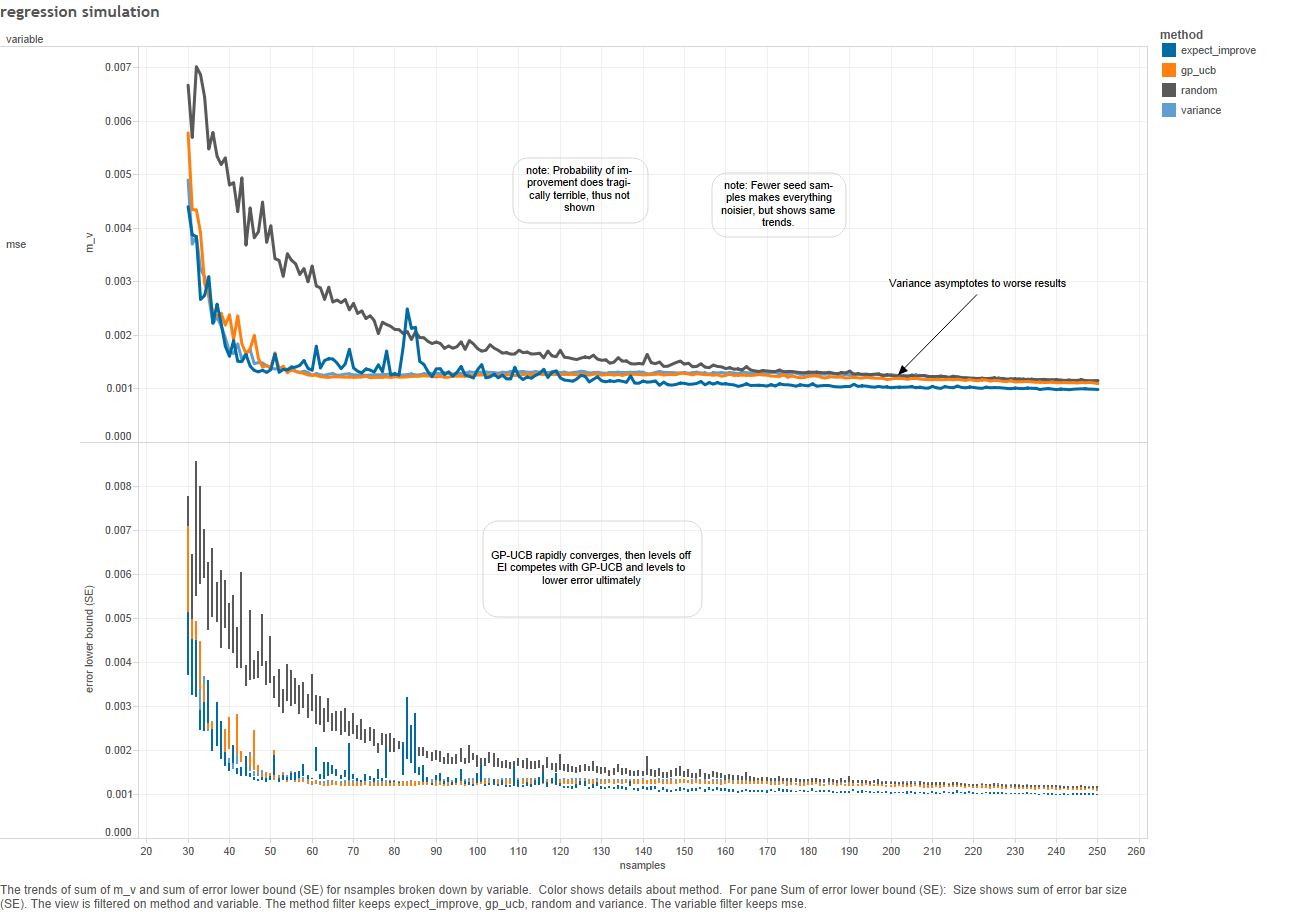
\includegraphics[width=\linewidth]{regression_simulation}
\caption{Regression simulation mean squared error vs number of samples used in training for different objective and acquisition function combinations. Decreasing values indicates increasing performance.}
\label{fig:reg_sim}
\end{figure}
%    all 3 methods do quite well
%    EI asmpytotes to slightly better results
In simulation all AL methods performed well except for PI (not shown as it distorts the graph scale) (Figure \ref{fig:reg_sim}).
As PI is a pure exploitation strategy it focuses on playtesting parameter settings that are highly certain.
Because we are tuning three parameters in a fine-grained space this makes it easy to find a bad set of parameters and fail to distinguish among many possible alternatives.
%
% TODO: PI might be bugged
%
Roughly 40 playtests were needed to tune the three parameters related to player performance against enemies when using GP-UCB, EI, or variance; random sampling require 175 playtests for comparable performance.
More playtests marginally improved AL performance.

% human
\begin{figure}[tbph]
\centering
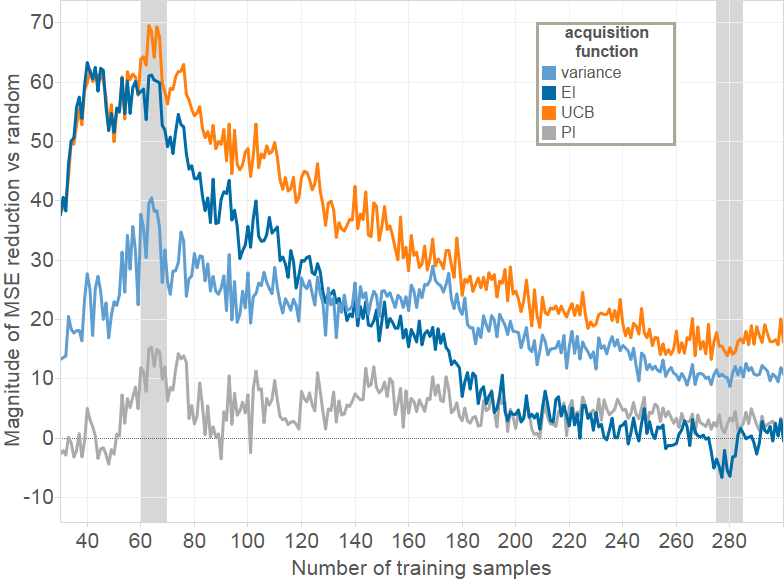
\includegraphics[width=\linewidth]{regression_experiment}
\caption{Regression human study mean squared error vs number of samples used in training for different objective and acquisition function combinations. Decreasing values indicates increasing performance.}
\label{fig:reg_expr}
\end{figure}
    % UCB and EI are only ones to do well
    % -- UCB remains at consistently high performance
    % -- EI gradually gets worse over time
    % why?
    % -- variance and PI do not capture exploration and thus have difficulty finding good results
    % -- UCB is able to temper exploration and exploitation over time, likely helping focus on best areas to test
In human studies GP-UCB and EI both performed well, other AL methods did not (Figure \ref{fig:reg_expr}).
We focus our analysis on the GP objective function as NE for regression was unable to outperform a random sampling approach which was worse than all GP method results.
Gaussian Processes were developed for regression settings so it is not surprising that neural networks---developed for classification---would show relatively poor performance.

Variance's low performance is explained by the tendency to focus on highly uncertain parameter settings---in a high-dimensional space it is easy to find many sets of uncertain bad parameters, leading to poorer performance.
Over time EI's performance gradually decayed while GP-UCB maintained better performance.
As more samples are gathered GP-UCB is better able to reduce exploration while EI eventually begins making poor playtest choices.
Approximately 60 samples were needed to train the successful AL methods to their peak performance; random sampling never achieved this level of performance on our data set.
Overall this is a clear demonstration that AL can enhance playtesting efficacy, perhaps beyond what would happen through simply A/B testing and collecting data.

% summary
Our regression experiments demonstrate the power of AL to reduce the amount of playtesting required.
Methods that balance exploration and exploitation---EI and GP-UCB---show the greatest efficacy across simulation and human studies.
These results make a strong case for AL applied to optimizing low-level in-game behaviors, such as difficulty in terms of in-game performance.


\subsection{Classification}
Our classification experiments show AL can be effective but is more challenging in subjective domains.
In simulation data AL methods---particularly entropy sampling---show significant improvements over random sampling.
% TODO : rerun w/new data subset to check if still bad
% if so, not sure whether to keep or admit weak results
% may want to hack on classifiers more or try other feature sets
Human data did not show strong improvements for AL methods and only marginal performance improvements for random sampling.
These results suggest AL works for preference learning when the domain can be modeled as a preference choice, but that our human data was not of this sort.


% simulation
\begin{figure}[tbph]
\centering
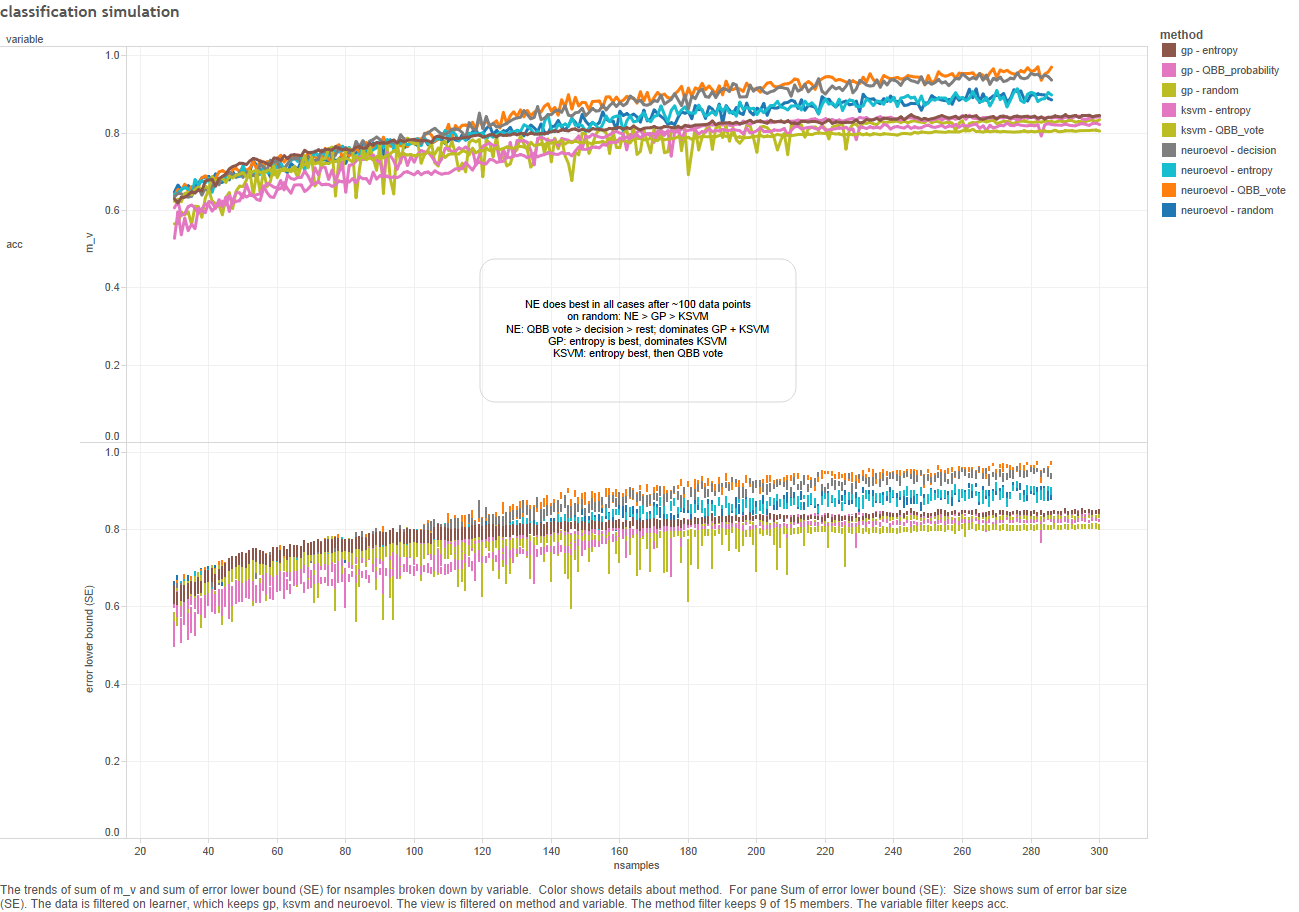
\includegraphics[width=\linewidth]{classification_simulation}
\caption{Classification simulation F1 score vs number of samples used in training for different objective and acquisition function combinations. Increasing values indicates increasing performance.}
\label{fig:cls_sim}
\end{figure}
    % GP random beats KSVM random -> GP is better able to model domain
    % GP entropy shows best trend -> focus on finding out where problems are
    % QBB models do moderately, but expensive to train -> best for high variance situations and model was not too high variance [cf Schein logreg]
    % NE most effective; esp QBB vote
    % NE random outdoes others
In simulation QBB vote and entropy sampling showed strong performance gains across all three objective functions (Figure \ref{fig:cls_sim}).
Previous work has found QBB models are best for high variance data sets \cite{schein2007:al-logreg-eval}.
Entropy sampling is also effective for high-variance situations.
The complexity of our simulation model made it a highly variable function to optimize and demonstrates the value of AL methods that can handle these situations.


% human
\begin{figure}[tbph]
\centering
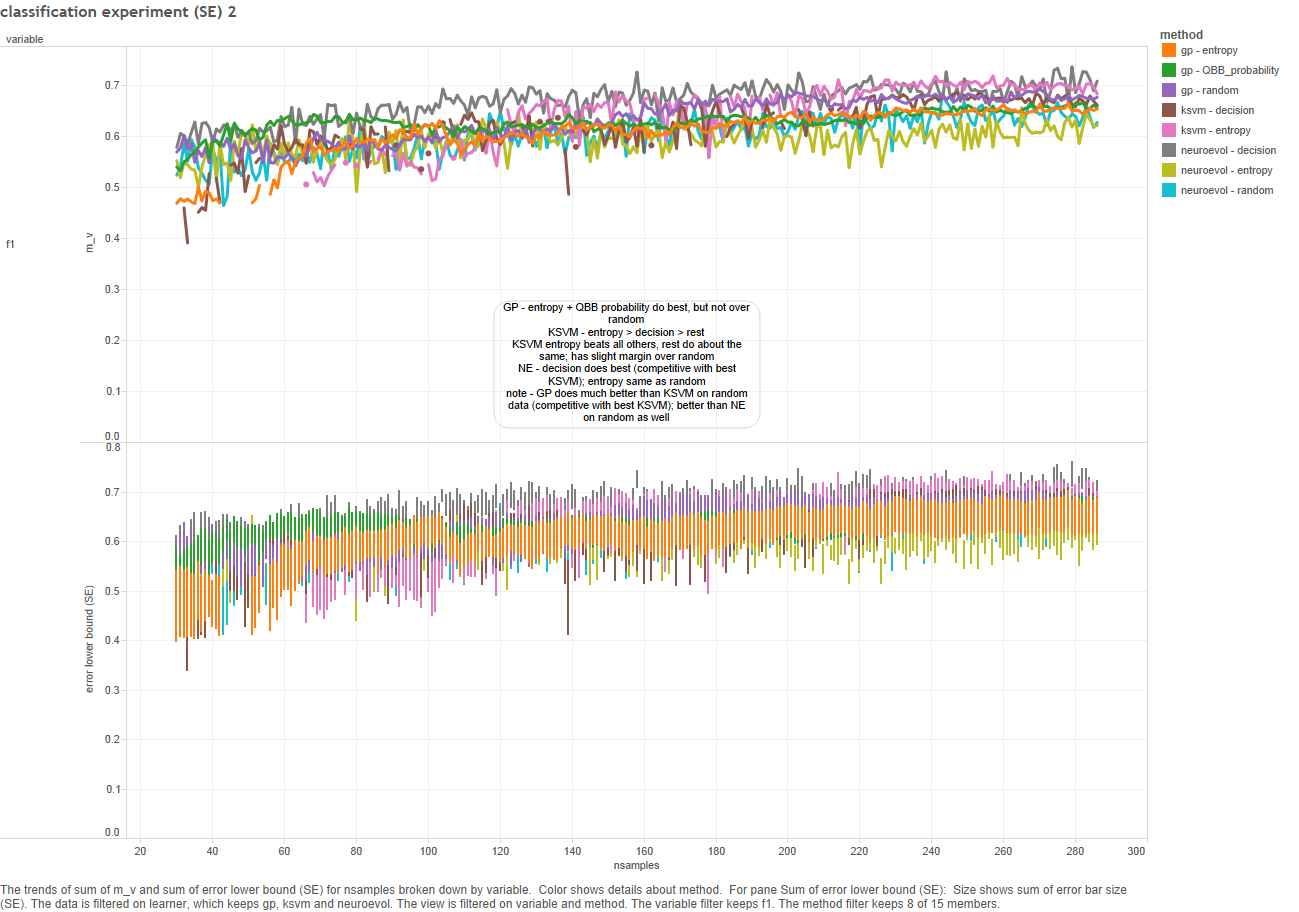
\includegraphics[width=\linewidth]{classification_experiment}
\caption{Classification human study F1 score vs number of samples used in training for different objective and acquisition function combinations. Increasing values indicates increasing performance.}
\label{fig:cls_expr}
\end{figure}
    % all methods roughly equal
    % GP random does well
    % GP random beats KSVM random -> GP is better able to model domain
    % no strong winners, domain was very hard
    % KSVM entropy is slightly better 
    % QBB models don't perform 
    % --> QBB + KSVM results suggest consistent domain but complex underlying model
    % only minor gains: ~160 samples to improve, little growth over random
In human studies only very specific acquisition and objective function combinations were able to show substantial improvements (Figure \ref{fig:cls_expr}).
Neural network optimization (NE) was unable to improve over random sampling.
These results are surprising given the efficacy of neural nets for preference learning in other contexts and merit additional investigations. % my hunch: fewer features makes it harder

Gaussian Processes showed initially strong learning (by 60 samples using QBB probability or vote), but random sampling reached competitive performance with more (160) samples.
Kernel SVMs showed the opposite trend: entropy showed strong performance only after reaching many samples (200).
Overall these results suggest that GPs are able to effective learn when few samples are available by using QBB acquisition functions to mitigate variance.
With a larger pool of samples KSVMs eventually become more effective, though GPs appear to converge to similar performance.

% summary
Our classification experiments demonstrate AL can reduce the amount of playtesting needed even for subjective features of a design such as control settings.
Reducing playtest costs, however, requires acquisition functions that mitigate the high variance inherent in subjective response data.






%%%%%%%%%%%%%%%%%%%%%%%%%%%%%%%%%%

\section{Conclusions}

% % note: can combine multiple aspects into single acquisition function, but then need additional complexity of learning how to balance objectives if not told directly; e.g. preference + performance

% % enable continuous model improvement

% % future: optimal experimental design (rafferty, chaloner); hcomp for more direct human participation





%%%%%%%%%%%%%%%%%%%%%%%%%%%%%%%%%%

\section{Acknowledgments}
% Eric Fruchter - or possible co-author


\bibliographystyle{abbrv}
\bibliography{../latex/lib}  % keeping lib in separate github project

\end{document}
